

\section{Results}
\label{sec_experimentalResults}
This section presents our experimental results and their interpretations, for
the protocols presented in \autoref{sec_protocols}, applied on the ensemble data
described in \autoref{sec_caseStudy}
% , which has been made
(publicly
available \cite{data}).


\subsection{Persistence curve study}



We applied protocol 1 using the persistence curves, on our ensemble dataset of Kelvin-Helmotlz instability (KHI) to verify the hypotheses of separation of the schemes (H1) and the independence of the orders (H2)(\autoref{Hypotheses}). 
The input parameters are setup as detailed in \autoref{sec_protocols}, generating 36 studies. The terrains and curves on
% Figure
\autoref{curv} illustrate the result for one configuration with a 5th order WENO-Z (\autoref{curv}.a), a 7th order WENO-Z (\autoref{curv}.c), a 5th order WENO-Z (\autoref{curv}.f) and a 5th order TENO (\autoref{curv}.h). For the scheme comparison, most of the averaged persistence curves for the TENO schemes (blue curves on \autoref{curv}g) are above the WENO-Z curves (green curves on \autoref{curv}g).
The integral difference, between the average curves, obtain results between $[-5.6,5.2]$ (\autoref{curv}.e), which demonstrates differences on the topology of the enstrophy between the interpolation methods as expected.
Hypothesis H1 is verified on the KHI ensemble dataset. For the study on the 
independence of orders, we see that the averaged persistence curves are often 
close (\autoref{curv}b). However the integral differences obtained for this 
study show larger values for the WENO-Z, \emph{i.e} in between $[-0.5, 8.1]$ 
(\autoref{curv}.d). This analysis highlights that orders play a more important 
role, in terms of topology of the vortices, for WENO-Z than for TENO. Moreover, 
we observe that this difference tends to increase at $t_2$ for both studies 
confirming that the flow is composed of a larger number of vortex as the 
simulation evolves. Hypothesis H2 is verified for the TENO solvers but not for 
the WENO-Z
% as discussed
% later 
% in
(\autoref{insights}).
 



\subsection{Outlier distance profile study}
\label{sec_KHIdistance}


% In order t
To verify the HLL isolation states in hypothesis H3 (\autoref{Hypotheses}) on our ensemble dataset, we implemented our protocol 2 (\autoref{sec_protocols}) based on the Wasserstein distance and the $L_2$-norm (\autoref{sec_topology}). For this study we apply protocol 2 where the time and the resolution are fixed. The parameters that vary are the schemes ($\times 2$), the orders ($\times 2$) and the solvers ($\times 5$) (\autoref{tab_parameters}) thus generating 20 cases. All the distances have been computed according to the protocol of the outlier distance profile. These distances are represented by a global distance matrix where a line represents the 20 configurations (Wasserstein \autoref{fig_KHIdistance}.a and $L_2-$norm \autoref{fig_KHIdistance}.h) compared to a the HLL solver choosen as the reference. The matrix view of \autoref{fig_KHIdistance}b and \autoref{fig_KHIdistance}g show the KHI terrains and the distances of all configurations to the HLL solver.

The study has been done for all time steps and all resolutions generating nine
$20\times 20$ 
distance matrices, for each distance. The histograms (Figs. 
\ref{fig_KHIdistance}.c and \ref{fig_KHIdistance}.e) 
% (\autoref{fig_KHIdistance}.c) and (\autoref{fig_KHIdistance}.e) 
show the average 
of these nine distance matrices for the Wasserstein distance and the 
$L_2$-norm, expressed in terms of percentage according to the distance of HLL 
to the other solvers (HLL being the reference at 100\%). In this case the 
percentage difference in distances to HLL are about 18\% 
(\autoref{fig_KHIdistance}.d) for the Wasserstein and 13\% for the $L_2$ 
(\autoref{fig_KHIdistance}.f). These large percentages confirm that HLL is a 
solver that behaves differently from others.
% More precisely, a
As it does not take
into account contact discontinuities, the interfaces between the vortices
are much less defined than with the other solvers, resulting in a different
number of vortices. From a physical point of view, this result confirms the 
isolation of HLL in all cases. From a topological point of view, it shows that 
the Wasserstein distance is the best at differentiating the HLL solver from the 
others (the distance gap is always bigger than the $L_2$). For this large study 
of 18 distance matrices $20\times 20$, the hypothesis H3 is verified. 

\begin{figure*}
 \centering % avoid the use of \begin{center}...\end{center} and use \centering
 \vspace{-1ex}
 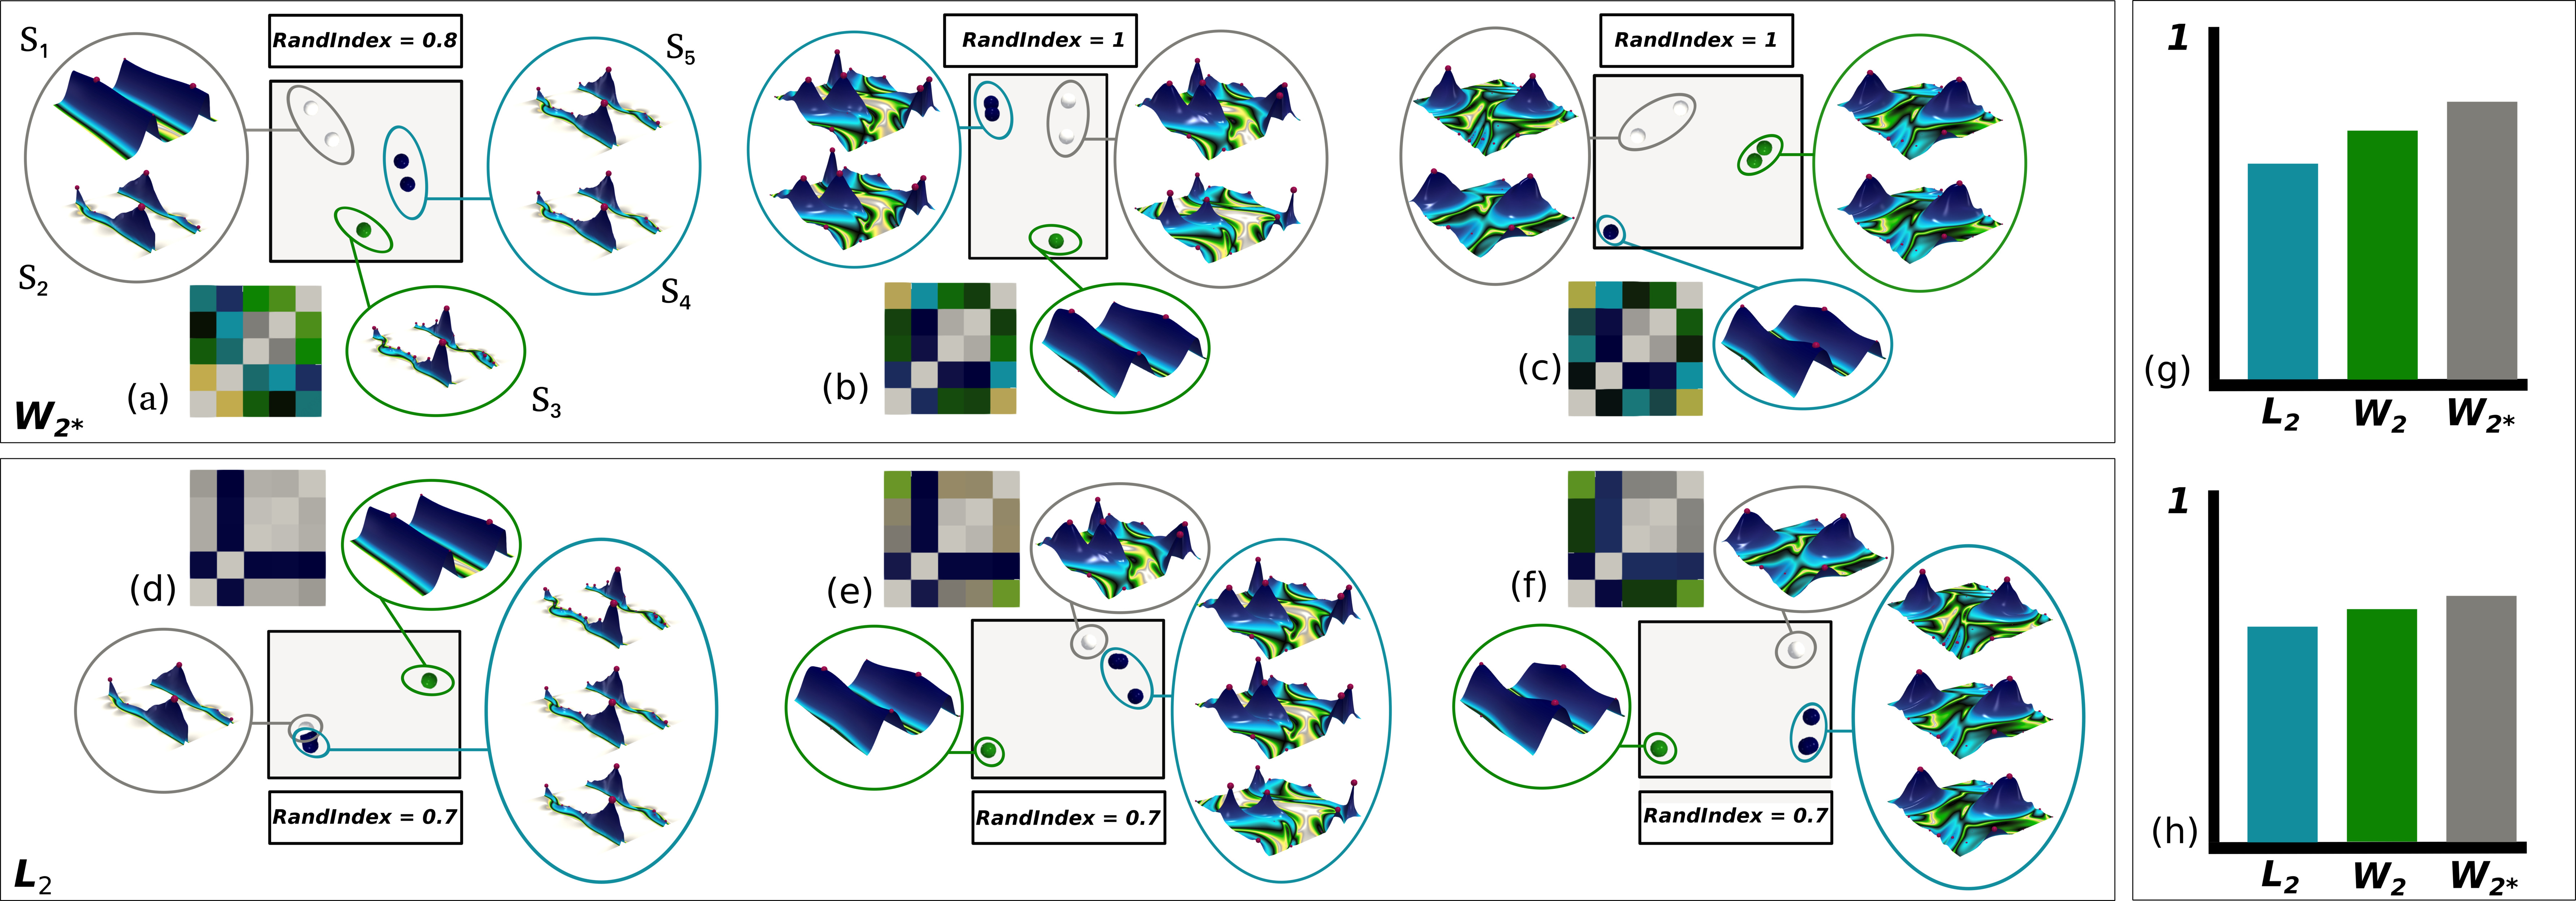
\includegraphics[width=\figureShrink\linewidth]{chapter4_topology_data_analysis/pictures/KHI_cluster.jpg}
 \mycaption{Comparison between the clustering on the Wasserstein metric space \cite{vidal_vis19} (top frame) and a clustering based on the traditional $L_2$ norm (bottom frame) for distinguishing FDS solvers from FTS solvers.
Point clouds at $t_0$, $t_1$,$t_2$ with a first order scheme at $256\times 256$.
The point cloud is a representation of the five scalar-fields in the distance
space colored according to the clusters obtained. The Rand Index are computed
with the five configurations $S_1$ (SLAU2), $S_2$ (HLL), $S_3$ (AUSM$^+$-UP),
$S_4$ (Roe), $S_5$ (HLLC). (g,h) Average Rand Index for all variations for the
high orders (bottom) and the first order (top).}
\label{fig_khi_cluster}
\end{figure*}


\subsection{Unsupervised classification study}
 \label{sec_khi_cluster}
To improve our understanding on the behavior of the solvers into our simulation code, we implemented protocol 3 on the unsupervised classification (\autoref{sec_protocols}) to verified the hypotheses H4 and H5 (\autoref{Hypotheses}). The goal is to identify the separation of FDS type solvers from the FTS type solvers (\autoref{sec_solvers}). We are interested in the low Mach reconstructions (\autoref{sec_solvers}). The challenge comes from the fact that small vortices are reconstructed on only a few cells. So, we implemented protocol 3 with the distances and clustering method detailed in \autoref{sec_protocols} leading to 5 simulation configurations (\autoref{tab_parameters}) with variable solvers. To focus on the small vortices we used a threshold of 0.38 persistence for the topological methods. On the KHI ensemble, we generated 36 clusters from the threshold persistence diagrams and obtain the Rand Index for all of them. \autoref{fig_khi_cluster}.a, \autoref{fig_khi_cluster}.b, \autoref{fig_khi_cluster}.c show the $W_2*$ clustering for the three timesteps and \autoref{fig_khi_cluster}.d, \autoref{fig_khi_cluster}.e, \autoref{fig_khi_cluster}.f for the $L_2$.

Histogram \autoref{fig_khi_cluster}.h shows the average Rand Index for the 
three methods with a value of 0.63 for $L_2$, 0.66 for $W_2$ and 0.71 for $W_2*$.
There is very little difference between the topological and geometric results 
and each of the methods struggles to get the right cluster. Hypotheses H4 and H5 
are not verified for high orders. However, to highlight the differences between 
solvers, it is necessary to use a reference reconstruction that barely captures 
small scale turbulence due to order dissipation (\autoref{sec_solvers}).
Thus, we applied protocol 3 (\autoref{sec_protocols}) on a more restricted 
dataset at order 1. Histogram \autoref{fig_khi_cluster}.g shows the average 
Rand 
Index at order 1 with the three methods leading to 0.63 for $L_2$, 0.71 for $W_2$
and 0.78 for $W_2*$. In this case, we notice that for any reconstruction, the 
topological methods obtain better clustering. Moreover, the study with order 1 
shows that the $W_2*$ method enhances solver isolation.
% of the solvers.
With this
high score of the Rand Index hypotheses H4 and H5 are verified with the first 
order. 

\subsection{Unanticipated insights}
\label{insights}

During the analysis of the persistence curves generated by our protocol 1, we found significant differences on the topology of the enstrophy between the orders for the WENO-Z. By increasing the order, we increase the accuracy of our calculation that generates more structures into the turbulent flow. On the other hand, there is no difference between the orders obtained with the TENO. This means that other ingredients in the TENO reconstruction play an important role in the computation of the turbulence such as the separation of the scales. In addition, the persistence curves also allowed us to observe that the WENO-Z schemes produce more numerical errors than the TENO. As presented in \autoref{sec_khi_cluster}, H4 and H5 hypotheses have not been verified for high orders. This means that the topological analysis does not capture the differences between the solvers. This may be due to the reconstructions which are accurate enough to calculate all velocities in the Kelvin-Helmholtz instability. 

\subsection{Limitations}
As discussed in \autoref{sec_KHIdistance}, in comparison to the $L_2$ norm, the Wasserstein distance
improvesthe separation of the HLL solver, but only by $5 \%$ (distance difference percentage). While this improvement may seem marginal, we would like to stress its significance given such challenging data,in particular with regard to the traditional approach based on kinetic energy, shown \autoref{energie}, where the five solvers can hardly be distinguished from each other.

Similarly, we can see that the Rand Index score for the three clustering
methods detailed in \autoref{sec_khi_cluster} are quite close to each other as
illustrated on \autoref{fig_khi_cluster}.h. These close scores are due to the 
interpolations schemes (\autoref{sec_simulation}) which cover up the differences 
between the different solvers.
In other words, the variations in vortex distributions induced by the choice of solver are too subtle, given the importance of the interpolation order on the outcome. As shown in \autoref{fig_khi_cluster} (top), we were still able to overcome this limitation by considering a
reconstruction that is not dedicated to turbulence, \emph{i.e.} an upwind scheme 
of order 1. This enabled us to exaggerate the impact of the solvers, thereby allowing us to
validate hypotheses H4 and H5 as reported in \autoref{sec_khi_cluster}.
